%%%%%%%%%%%%%%%%%%%%%%%%%%%%%%%%%%%%%%%%%%%%%%%%%%%%%%%%%%%%%%%%%%%%%%%%%%%%%%%%%%%%%%%%%%%%%%%%%%%%%%%

\documentclass[rmp,aps,superscriptaddress,floatfix]{revtex4-2} 
\usepackage{graphicx}
\usepackage{xcolor} 
\usepackage{amsmath}
\usepackage{amssymb} 
\usepackage{natmove}
\usepackage{natbib}
\usepackage{hyperref} 
\usepackage{bm}

%%%%%%%%%%%%%%%%%%%%%%%%%%%%%%%%%%%%%%%%%%%%%%%%%%%%%%%%%%%%%%%%%%%%%%%%%%%%%%%%%%%%%%%%%%%%%%%%%%%%%%%

\begin{document}

\title{On the Origin of Shrimpoluminescence}

\author{Tyler C. Sterling}
\email{ty.sterling@colorado.edu}
%\affiliation{Department of Physics, University of Colorado at Boulder, Boulder, Colorado 80309, USA}

\date{\today}

\begin{abstract}
shrimpity shrimp shrimp shrimp. abstract abstract abstract abstract abstract abstract abstract abstract abstract abstract abstract abstract abstract abstract abstract abstract abstract abstract abstract abstract abstract abstract abstract abstract abstract abstract abstract abstract abstract abstract abstract abstract abstract abstract abstract abstract abstract abstract abstract abstract abstract abstract abstract abstract abstract abstract abstract abstract abstract abstract abstract abstract abstract abstract abstract abstract abstract abstract abstract abstract abstract abstract abstract abstract 
\end{abstract}

\maketitle

%\listoffigures
%\listoftables
%\tableofcontents

%%%%%%%%%%%%%%%%%%%%%%%%%%%%%%%%%%%%%%%%%%%%%%%%%%%%%%%%%%%%%%%%%%%%%%%%%%%%%%%%%%%%%%%%%%%%%%%%%%%%%%%

%\emph{Frequently Used Abbreviations}
%\begin{itemize}
%    \item SL: sonoluminescence
%    \item SBSL: single-bubble sonoluminesence
%    \item MBSL: multi-bubble sonoluminescence
%\end{itemize}


\section{Introduction}
Snapping shrimp, like our cute friend in Fig. \ref{fig:shrimp_claw} (left), have long been known to produce cavitating bubbles by \emph{snapping} their claws \cite{versluis2000snapping,lohse2001snapping,tang2019bioinspired}. They have a strong appendage (the \emph{dactyl}) in thier claw [Fig. \ref{fig:shrimp_claw} (center)] that is used to create a very high-velocity jet of water. The low pressure region in the jet's wake forms a bubble [Fig. \ref{fig:shrimp_claw} (t=0 ms)] that, among other things, produces an exceptionally loud noise when it collapses. The sound (i.e. the pressure wave) produced by even a \emph{single} shrimp's snap is detectable over a mile away \cite{everest1948acoustical}. The noise produced by groups of shrimp is so intense that the U.S. Navy used them as ``sonar-camoflauge" in the Pacific ocean during World War II \cite{versluis2000snapping}. 

\begin{figure}
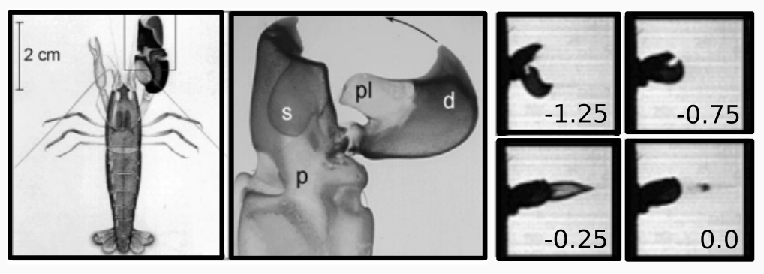
\includegraphics[width=0.9\linewidth]{figs/shrimp_claw.pdf}
    \caption{(left) Snapping shrimp (\emph{Alpheus heterochaelis}). (center) Blown-up view of the shrimp's claw. The \emph{plunger} (pl) on the \emph{dactyl} (d) rapidly enters the \emph{socket} (s), ejecting a high-velocity jet of water. The water ejection and subsequent bubble formation and, finally, bubble collape (at t=0) are shown on the right. The units are ms. Adapted from ref. \cite{versluis2000snapping}}
\label{fig:shrimp_claw}
\end{figure}

The shrimp were not patriots helping the war-effort, however; they snapped for food. The shock-wave produced by the cavitating bubble is used to stun and even kill prey \cite{versluis2000snapping}. If the shrimp's prey had very sensitive eyes (and also were not dead) they might notice a flash of light is also produced through an effect referred to as ``shrimpoluminescence" in the case of the pistol shrimp \cite{lohse2001snapping}, but more generally known as \emph{sonoluminescence}.

Sonoluminescence (SL) is more precisely defined as the process by which a ``driven gas bubble collapses so strongly that the energy focusing at collapse leads to light emission" \cite{brenner2002single}. Sonoluminescence comes in two forms: (i) single-bubble sonoluminescence and (ii) multi-bubble sonolumiscence. The disticntion is self-explanatory: multi-bubble sonolumiscence (MBSL) consists of  ``the simultaneous creation and destruction of many seperate, individual cavitation bubbles" \cite{crum1994sonoluminescence,brenner2002single}, whereas in single-bubble sonoluminescence (SBSL), rather obviously, only a single bubble is present \cite{gaitan1992sonoluminescence}. The discovery of MBSL predates SBSL by $\sim$60 years but due to the more-or-less random and fleeting nature of the bubbles, SL in general wasn't well studied until the early 1990's when it was discovered that single bubbles could be created and periodically driven to produce light very high precisions \cite{crum1994sonoluminescence,gaitan1990experimental,gaitan1992sonoluminescence,brenner2002single}. We will discuss MBSL breifly later, but for now it suffices to say that nearly all theoretical and experimental progress has been made using SBSL, with some authors even calling it ``the hydrogen atom of sonoluminescence" \cite{lohse2018bubble,crum1994sonoluminescence}.

The discovery of SBSL created a rush of effort to explain the phenomena with arguments ranging from the simplest models \cite{} to more exotic explanations based of quantum field theory \cite{schwinger1993casimir,eberlein1996sonoluminescence,liberati2000sonoluminescence}.


But besides shrimpoluminescence, why is SL interesting? Well, at a glance, it is not obvious why SL occurs. The acoustic wave in the liquid displaces molecules on the order of nanometers, costing an elastic energy of  $\sim1\times 10^{-12}$ eV/molecule while emitting visible light (through e.g. electronic transitions) costs an energy $\sim1$ eV/molecule \cite{lohse2018bubble,crum1994sonoluminescence}... there is a 12-orders-of-magnitude concentration of energy. That is huge! After a moments thought, however, the massive energy focusing is not that surprising. For example, the energy in the shock wave produced by a cavitating bubble, regardless of the light production, has been known to damage ship propellers since atleast 1917 when Lord Rayleigh's gave the first rigorous treatment of caviating bubbles \cite{gaitan1990experimental}. A heurestic argument goes like this: \cite{plesset1949dynamics}. 

So again, why is the light emmission interesting? In short, after 3 decades of studying SBSL, the mechanism of light production is still not understood. 

The excitment wasn't restricted to academics however, with SBSL catching Hollywood's attention leading to an unpopular movie called \emph{Chain Reaction} where t


So again, why is the light emmission interesting? After 3 decades of studying SBSL, the physical mechanism of light production in SL is still not understood. This can be seen by glancing at the literature and noticing that there are many recent papers with different arguments for \emph{where} the light comes from \cite{borisenok2020mechanisms,flannigan2013non,flannigan2012temperature,tatartchenko2017sonoluminescence}. We emphasive ``where" since it's not even certain if the light is \emph{surface} or \emph{volumetric} emission, i.e. it is literally not known \emph{where} the light comes from \cite{}. 

... and others stating that ``SBSL has become a rather sophisticated testing ground for the ability of mathematical models and numerical simulations to explain detailed experimental data from a complicated physical process" \cite{brenner2002single}.


The goal of this paper is to catch the reader up on recent efforts to explain SBSL. While the author of this paper is particularly excited about shrimpoluminescence, it is important to stress that this work will focus on SBSL in general. It is apparently simpler to create and characterize SBSL in the laboratory without involving shrimp (for example, using shrimp involves convinving them to snap by tickling them \cite{lohse2001snapping,versluis2000snapping,lohse2018bubble}), so practically all work to study SL has not involved shrimp ( ... with notable exceptions \cite{tang2019bioinspired}).

\section{Historical Overview}

\section{What do we know?}
\subsection{The Bubble Wall}
\subsection{Experimental Results}
what conditions are necessary for light emission (i.e. what is the phase space \cite{lohse2018bubble}):
\begin{itemize}
    \item Ar content
    \item driving frequency
    \item P$_{max}$
    \item ...
\end{itemize}

\section{What don't we know}
\subsection{The Bubble Wall (Again)}
\subsection{Experimental Anomalies}


\section{Let there be light!}
\subsection{Thermal Arguments}
\subsection{Electric Arguments}

\subsection{The Casimir Effect}
\subsection{The Casimir Argument}


\section{Summary}

\section{Acknowledgments}





\newpage 

\section{random notes}

argon flash: a method of 'imaging explosions' similar to why argon is more useful for SBSL. argon has no internal DOF whereas air (i.e. N2, O2, water vapor) does and energy from explosions is absorbed dissociating bonds. argon, instead, becomes 'hotter' and emits more light, making photographing explosions easier. see wikipedia article "argon flash"



some dickheads 3d printed a shrimp claw and it also shrimpoluminesces \cite{tang2019bioinspired}

apparently a shitty movie called 'Chain Reaction' with Keanu Reeves was centered around the premise of MBSL as a means of clean energy production. it was based on the speculation that temperatures inside the bubbles ciould reach up to millions of Kelvin and lead to fusion. this was debunked by Prosperetti (see the pop sci article \cite{chainreaction}). He points out that the temp is speculative and is based on assumptions of a perfect sphere collapsing. he notes that its probably not spherical when light is produced and even points out that groups have tried to produce fusion power by intentionally collapsing gas filled micro baloons with lasers... and failed. Tatartcheceko also shows that this is horsehit \cite{tatartchenko2017sonoluminescence}. in this article, Prosperetti also explains how a 'jet' of water whooshing across the bubble could be going faster that 4000 mph, fast enough to cause non-netwownian fracturing of the water leading to light producuction through (apparently) the same mechanism of light emession when ice or wint-o-green mints are snapped in half... huh. this is good introduction fodder. need to find the primary lit. 

for fusions, also see wikipedia article on 'bubble fusion' and 'Rusi P Taleyarkhan'. Ruse was some asshole prof at purdue that claimed fusion occured inside cavitating bubbles, but it was later found out that the faked data and interfered with peer reviews leading to him being fucking fired.

\emph{heurestic explanation of bubble trapping given by Brenner in \cite{chainreaction}.}: the bonds between molecules in a fluid are very strong, so instead of 'tearing', the fluid stretches. however, if there is a bubble present, the local dialation of the fluid can change the bubbles diameter by $\sim$ 1000 times to avoid breaking bonds at the interface between bubble and fluid. But when the compression waves comes by, the 'gas' in the bubble, which has boiled due to low pressure, offers very little resistance to compression. the wave compresses the bubble rapidly, which spikes the temp in the gas to incandescent temperatueres. this heuristic explanation is on-track with Crum \cite{crum1994sonoluminescence} below.

\section{1st discovery}
MBSL was discovered first. its (obviously) hard to create and control single bubbles so this wasnt feasible until the 1990s, attributed to Gaitan (see below). allegedly, it was Marinesco et al \cite{marinesco1933actions} that discovered MBSL in 1933 (according to \cite{gaitan1990experimental} below and to \cite{tatartchenko2017sonoluminescence}) but I cant find this paper (or understand it since its in french). Other sources (e.g.. wikipedia, \cite{tatartchenko2017sonoluminescence,crum1994sonoluminescence}) credit Frenzel et al \cite{frenzel1934luminescenz} as the discoverers. I cant German or find this paper either, but in anycase, Tatartchenko summarized thier discovery: Freznel and coworkers were trying to speed up photo development by 'insonating' i.e. subjected developer-fluid to sound. they found that when they immersed photo-plates or whatever in the fluid, it became 'foggy' and overexposed, as if subjected to diffuse light. A bunch of other papers followed up on this. get the deets from \cite{gaitan1990experimental} below. 

Update: Brenner \cite{brenner2002single} consisely summarizes the history: Marinesco notes the photographic plates fogs in an ultrasonic bath \cite{marinesco1933actions} and Frenzel et al \cite{frenzel1934luminescenz} deliberately studied the light emission. According to brenner, no one was surprised by this since it was already known that cavitating bubbles fuck shit up.

SBSL was discovered by Gaitan \cite{gaitan1990experimental,gaitan1992sonoluminescence} etc. who trapped a single air bubble in a water filled flask using piezoacoutics stuck to the outside. (note: the trapping force is called \emph{Bjerknes force}, refs in \cite{lohse2018bubble}).

\section{notes from \cite{crum1994sonoluminescence}}
pop sci type of magazine article. Gives heurestic expanation: When an intense sound field is produced within a liquid, microscopic cavities of gas or vapor can be generated when the liquid fails under tensile stress. The subsequent acoustic compression cycle forces these cavities to collapse violently, which results in a remarkable concentration of mechanical energy, estimated to be as high as 12orders of magnitude (refs are given too). Also notes that MBSL is very hard to study since the bubbles occur randomly and transiently. Describes SBSL as the \emph{hydrogen atom of sonoluminescence}.also discusses that attempts to measure the (time) interval over which light is produced have found it be less than $\sim$50 ps which is 1/1000 times smaller than theory predicts. They also found the light to be more 'stable' than the acoustic generator, i.e. more regular with more controlled intervals. an old but probably still relevant result. mentions a neat claim that the conditions of the gas at the center of the bubble are probably more like a metal than a gas. \textcolor{red}{hell, this article basically summarizes all of the anomalies present in 1994. a very good resource.}

\section{notes from ref \cite{lohse2018bubble}} 
SBSL was discovered by Giatan et. al. in 1990s at U. Mississippi \cite{gaitan1990experimental,crum1994sonoluminescence,gaitan1992sonoluminescence} (note, \cite{gaitan1992sonoluminescence} has $\sim$1000 citations..). The SBSL experiments were done by sticking peizoacoustic transducers to the outside of a water filled glass. the 'Bjerknes' force trapps the bubble and the acoustic wave drives its expansion/collapse. What Gaitan saw was that even the single bubble emits light. Wow! This was baffling since 'acoustic energy' \textcolor{red}{(i dont understand this)} is on the order of $\sim10^{-12}$ eV/molecule while visible light is $\sim1$ eV. NVM: I do get this. Typical acoustic waves, e.g. in air, only displace molecules on the order of nanometers, which aquires an elastic energy gaine between molecules of $\sim10^{-12}$ eV/molecule: certainly not enough to excite an electronic transition. 

This paper refs the review by Propsperetti: \cite{plesset1977bubble}. This paper gives EOM for the bubbles radius, the so called \emph{Plesset-Rayleight} equation which I have seen everywhere related to bubbles. Talks about solving it, some other crap related to bubble dynamics. this requires a detailed re-read.

Later in the paper, also revisists snapping shrimp.

\section{notes from ref \cite{prosperetti2004bubbles}}
has shit tons of relevant math. take a look. a pretty paper overall


\section{notes from \cite{gaitan1990experimental}}
disseration by Giatan who is credited with discovering SBSL. says apparently SL was discovered in 1933. need to go read this crap. Apparently this was by Marinesco et. al. in 1933. Zimakov tried to explain it in 1934 and concluded that the light was due to electric discharge between vapor cavities and the glass container. Frenzel and Schultes in 1935 instead claimed it was from friction between cavitating bubbles and the water. Chamber in 1936 studied SL in other nonwater liquids. Chamber also postulated the light was from 'tribolumiscence' which occurs when the crystalline structure of the liquid-bubble lattice collapses? Apparently somthing similar occurs in real crystals. ... shit, a bunch more models are given. give this dis. a lot of attention.

also says caviation was predicted by 'Euler' in 1754: \emph{if the velocity of a fluid is high enouhg, negative pressures can form and the liquid can 'break'.} the 'breaking' was called cavitation in 895 by R.E. Froude, whoever the fuck this is, when studying bubbles near propellers. Rayleigh, unsurpisingly, was the first to give a rigorous theoretical treatment of cavitation in 1917.

\section{notes from \cite{brenner2002single}}
defines SBSL as ``Single-bubble sonoluminescence occurs when an acoustically trapped and periodically driven gas bubble collapses so strongly that the energy focusing at collapse leads to light emission". 

\section{QED}
the ref \cite{liberati2000sonoluminescence} has lots of good refs. they have follow up papers extending Schwingers papers (which are refd therein) and referencing a bunch of other relevant literature. I should look for refs citing Schwingers paper to try to figure out the modern state of the art of this thin.

\section{Modelling}
in the ref \cite{schanz2012molecular}, they use MD to modelling the equation of state for a collapsing bubble. they calculate the temperature and study the conditions for emitting light.

\section{Refs. to different arguments}
ref \cite{didenko2000molecular} gives examples of other origin theories (molecular excited states, black-body radiation, bremsstrahlung, ion-electron recombination, confined electrons)


%%%%%%%%%%%%%%%%%%%%%%%%%%%%%%%%%%%%%%%%%%%%%%%%%%%%%%%%%%%%%%%%%%%%%%%%%%%%%%%%%%%%%%%%%%%%%%%%%%%%%%%

\bibliography{../ref}

\end{document}
